\section{Durchführung}
\label{sec:Durchführung}
Bei dem im Versuch verwendeten $\alpha$-Strahler handelt es sich um $\ce{^241_95\text{Am}}$, welches mit einer Halbwertszeit von $T_{1/2} = 458 a$:
\begin{equation}
\ce{^241_95\text{Am}} \longrightarrow \ce{^237_93\text{Np}} + \ce{^4_2\text{He}}
\end{equation}
zerfällt.

\begin{figure}[H]
    \centering
    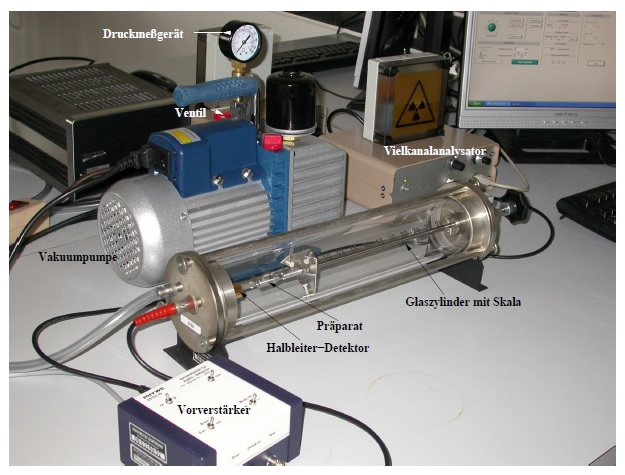
\includegraphics[width=0.5\textwidth]{build/Abb1.jpg}
    \caption {Versuchsaufbau zur Messung der Reichweite von Alphastrahlung\cite[2]{V701}.}
    \label{fig:Abb1}
\end{figure}

Wie in \autoref{fig:Abb1} zu sehen, wird der Versuch aufgebaut.
Das Präparat befindet sich auf einer beweglichen Halterung in einem evakuierbaren Glaszylinder. Im Glaszylinder befindet sich 
außerdem ein Detektor. Mit der beweglichen Halterung kann der Abstand $x_0$ zwischen Präparat und Detektor verändert werden.
Bei dem Detektor handelt es sich um einen Halbleiter-Sperrschichtzähler, der ähnlich wie eine in Sperrichtung betriebene Diode
funktioniert. Sobald ein Alpha-Teilchen auf den Detektor trifft enststeht ein Elektronen-Loch-Paar in der Verarmungszone, wodurch
ein Stromimpuls entsteht. Dieser wird durch einen Vorverstärker verstärkt und an einen Vielkanalanalysator weitergeleitet.
Die Auswertung des Vielkanalanalysators erfolgt über ein Computerprogramm.

Vor der Messung muss die Diskriminatorschwelle am Vielkanalanalysator eingestellt werden um Rauschen vom Verstärker zu unterdrücken, welches das Ergebnis verfälsche  würde.
Außerdem wird der Glaszylinder evakuiert.
Das Präparat wird auf einen Abstand $x_0= \qty{1.7}{\centi\meter}$ zum Detektor platziert und die Messung gestartet.
Der Messzeitraum beträgt jeweils $\qty{120}{\second}$. Der Druck im Glaszylinder wird um $\qty{50}{\milli\bar}$ erhöht und die Messung wiederholt.
Dieses Verfahren wird so lange wiederholt bis im Glaszylinder wieder Normaldruck herrscht.
In einer Tabelle werden der Druck $p$, die Zählrate $N$ und der Kanal des Energiemaximums notiert.
Der Abstand $x_0$ wird auf $x_0= \qty{3.0}{\centi\meter}$ vergrößert und die Messung erneut durchgeführt.


Anschließend soll die Statistik des radioaktiven Zerfalls überprüft werden,
indem bei vollkommen evakuiertem Zylinder $100$ Messungen zu je $\SI{10}{\second}$ durchgeführt werden, in denen die Anzahl der Zerfälle aufgenommen wird.
Danach werden hieraus die Varianz und der Mittelwert errechnet und mit einer Gauß- und Poissonverteilung verglichen. 